\chapter{Evaluation}
\label{evaluation}
%DELETEME: The evaluation chapter is one of the most important chapters of your work. 
%Here, you will prove usability/efficiency of your approach by presenting and interpreting your results. 
%You should discuss your results and interprete them, if possible. 
%Drawing conclusions on the results will be one important point that your estimators will refer to when grading your work.
This chapter comprises two sections:
the first presents the results from the experiments of chapter \ref{maintwo},
the second discusses and interprets these results.


%###################################################################################
%###################### Results             ########################################
%###################################################################################
\section{Results}
\label{results}
\providecommand{\gfxwidth}{}\renewcommand{\gfxwidth}{0.8\textwidth}
%\paragraph*{Experiment 1}
This section presents the results from the four experiments conducted.
This includes, for experiment 1 and 3, the data aggregation statistics of the imitation learning process
and, for all experiments, the loss trends through the imitation/supervised learning process
and the racetrack completion shares over the maximum drone speeds from the race tests.


Table \ref{tab:e1_data} shows the data aggregation statistics of the imitation learning 
process for the variants of experiment 1. 
\begin{table}[h]
    \caption[
        Data aggregation of experiment 1
    ]{
        Data aggregation of experiment 1
        \label{tab:e1_data}}        
    \centering
    \begin{tabular}{|c|r|r|r|r|r|} 
        %\hline
        \cline{2-6}
        \multicolumn{1}{c|}{}
        &F1
        &F2
        &R1
        &R2
        &R3
        \\\hline
        Learning completed
        &No
        &No
        &Yes
        &Yes
        &Yes
        \\\hline
        %
        \# Rollouts
        &297
        &208
        &114
        &136
        &178
        \\\hline
        \# Training samples
        &75,939
        &28,814
        &18,083
        &20,823
        &28,005
        \\\hline
        \# Validation samples
        &1,552
        &569
        &418
        &408
        &598
        \\\hline
    \end{tabular}
\end{table}
While all three recurrent variants (R1, R2 and R3) 
completed the imitation learning process, 
both feedforward variants (F1 and F2) stopped making progress and 
failed this task. The learning process of F1 (or F2) was terminated at the 
47th (72th) repetition of the rollout combination with a maximum drone speed 
of 5 m/s (10 m/s) and the last margin-threshold pair of (1.0 m, 1\%). 
Consequently, F1 completed about 2/3 of the learning rollout combinations, 
whereas F2 completed all but the last combination. In the incomplete learning process, 
both feedforward variants rolled out more often and collected more data than all 
three recurrent variants in the complete learning process. F1 performed the most 
rollouts with 297 and aggregated the most data with 75,939 training and 1,552 validation 
samples. F2 follows by a wide mar-gin with 208 rollouts and 28,814 training and 
569 validation samples. In third place is F3 with 178 rollouts and only slightly 
fewer data with 28,005 training and 598 validation samples. R1 (and R2) performed by 
far the least rollouts with 408 (418) and aggregated by far the least data with 
18,083 (20,823) training and 418 (408) validation samples.






Figure \ref{fig:e1_learn} shows the 
training and the validation losses
over the epochs of the imitation learning process 
for the variants of experiment 1.
\begin{figure}
    \centering
    \subfloat[
        Feedforward variants
    ]{
        \label{fig:e1_learn_feedforward}
        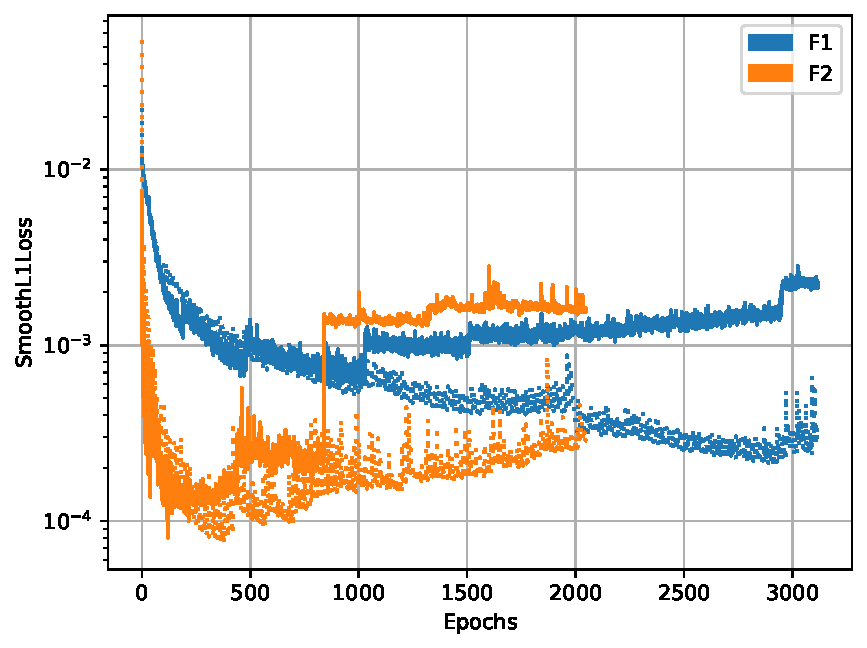
\includegraphics[width=\gfxwidth]{own/results_e1_learning_feedforward.pdf}
    }
    \hspace*{0cm}
    \par
    \subfloat[
        Recurrent variants
    ]{
        \label{fig:e1_learn_recurrent}
        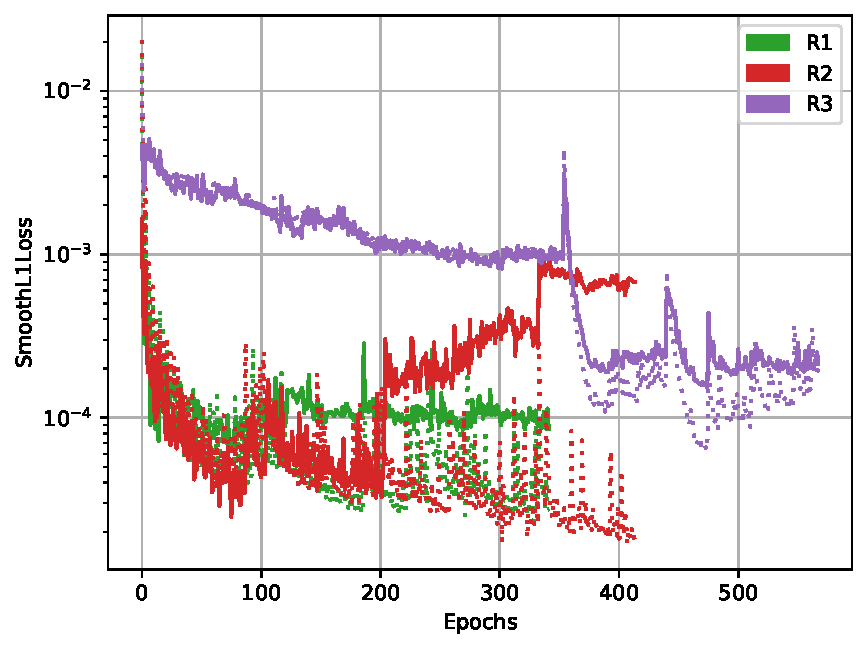
\includegraphics[width=\gfxwidth]{own/results_e1_learning_recurrent.pdf}
    }
    \caption[
        Training and validation losses of experiment 1
    ]{
        Training (dotted) and validation (solid) losses of experiment 1
        \label{fig:e1_learn}
    }
\end{figure}
The training or the validation loss of a variant is calculated with the SmoothL1Loss\footnote{
    \url{https://pytorch.org/docs/stable/generated/torch.nn.SmoothL1Loss.html}, accessed on \today
}
function on the training or validation dataset aggregated by that variant.
The figure displays the feedforward and the recurrent variants separately,
because the feedforward variants performed much more epochs than the recurrent variants in the learning process.
While F1 and F2 went through about 3000 and 2000 epochs, respectively,
R1, R2 and R3 required about 350, 400 and 550 epochs, respectively.
At the end of the learning process,
the feedforward variants achieve roughly the same losses on their aggregated data,
which are higher than the final losses of the recurrent variants.
F1 has a final training and validation loss of 
approximately $2.6\times 10^{-4}$ and $2.2\times 10^{-3}$.
F2 has a slightly higher, final training and a slightly lower, final validation loss of approximately
$2.9\times 10^{-4}$ and $1.6\times 10^{-3}$.
R1 has the second lowest, final training and the lowest, final validation
loss of approximately $2.7\times 10^{-5}$ and $8.6\times 10^{-5}$.
R2 has the lowest final training loss and 
the highest validation loss among the recurrent variants 
of approximately $1.8\times 10^{-5}$ and $6.7\times 10^{-4}$.
R3 has a final training and validation loss of approximately $2.0\times 10^{-4}$ and $2.1\times 10^{-4}$,
which are the closest final losses to each other.
From the lowest to highest,
the approximate ratios of validation to training losses are 
1.1 for R3,
3.2 for R1,
5.5 for F2,
8.5 for F1 
and 37.2 for R2.


Figure \ref{fig:e1_rcs} shows the racetrack completion shares (RCS)
over the maximum drone speeds of the race tests for the variants of experiment 1.
\begin{figure}
    \centering
    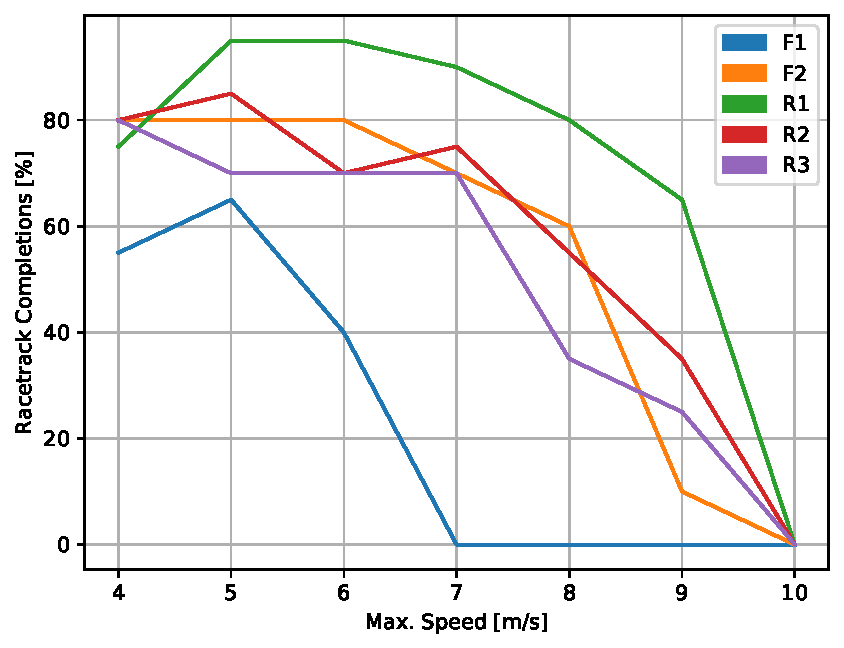
\includegraphics[width=\gfxwidth]{own/results_e1_racing.pdf}
    \caption[
        Racetrack completion shares of experiment 1
    ]{
        Racetrack completion shares of experiment 1
    \label{fig:e1_rcs}}
\end{figure}
The RCS of a variant is the share of the rollouts 
where the variant completed the racetrack
in all rollouts conducted with the same maximum drone speed in the race test of that variant.
For all variants, there is a tendency for the RCS to decrease with higher maximum speeds.
This culminates in the fact that no variant completed any racetrack 
for the highest maximum drone speed tested of 10 m/s.
At the maximum drone speed of 9 m/s, all three recurrent variants
perform better than the feedforward variants.
Over all maximum speeds, F1 has by far the lowest RCS,
which is roughly 50\% for lower speeds from 4 to 6 m/s
and 0\% for faster speeds from 7 to 10 m/s.
F2, R2 and R3 have roughly the same RCS over the tested maximum speeds,
which ranges from 70 to 85\% for maximum speeds from 4 to 7 m/s
and for higher maximum speeds decreases almost linearly to 0\% for 10 m/s.
The RCS of R1 is about the same as F2, R2 and R3
for the maximum drone speed of 4 m/s.
For maximum speeds from 5 to 9 m/s, however,
it is approximately 20 percentage points higher.





%\paragraph*{Experiment 2}
Figure \ref{fig:e2_learn} shows the 
training and the validation losses
over the epochs of the supervised learning process for the variants of experiment 2.
\begin{figure}
    \centering
    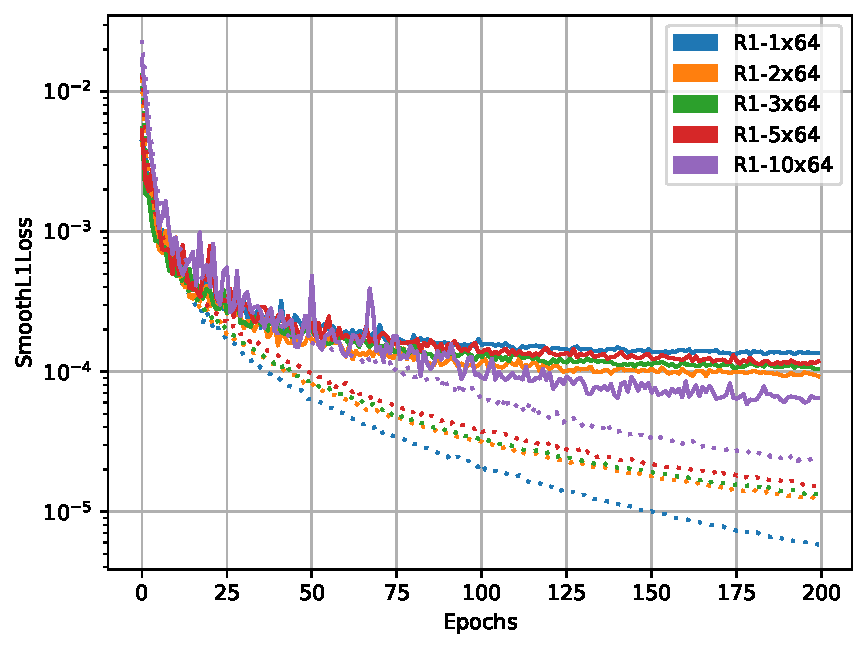
\includegraphics[width=\gfxwidth]{own/results_e2_learning.pdf}
    \caption[
        Training and validation losses of experiment 2
    ]{
        Training (dotted) and validation (solid) losses of experiment 2
    \label{fig:e2_learn}}
\end{figure}
The training or the validation loss of a variant is calculated with the SmoothL1Loss1 function 
on the final training or validation dataset of R1 in experiment 1.
All variants train for 200 epochs.
The single-layer GRU variant (R1-1x64)
achieves the lowest final training and the highest final validation loss
of approximately $5.8\times 10^{-6}$ and $1.4\times 10^{-4}$.
The 10-layer GRU variant (R1-10x64),
which has the most GRU layers in experiment 2,
achieves the highest final training and the lowest final validation loss
of approximately $2.3\times 10^{-5}$ and $6.5\times 10^{-5}$.
The variants in between (R1-2x64, R1-3x64 and R1-5x64)
achieve roughly the same final training and the same final validation loss
of approximately $1.3\times 10^{-5}$ and $1.0\times 10^{-4}$.
Consequently, from lowest to highest, the approximate
ratios of validation to training losses are 2.8 for R1-10x64, 7.7 for R1-2x64, R1-3x64 and R1-5x64
and 24.1 for R1-1x64.
The validation loss of R1-10x64
converges with a higher fluctuation than the validation losses of the other variants.


Figure \ref{fig:e2_rcs} shows the RCS over the maximum drone speeds
for the variants of experiment 2.
\begin{figure}
    \centering
    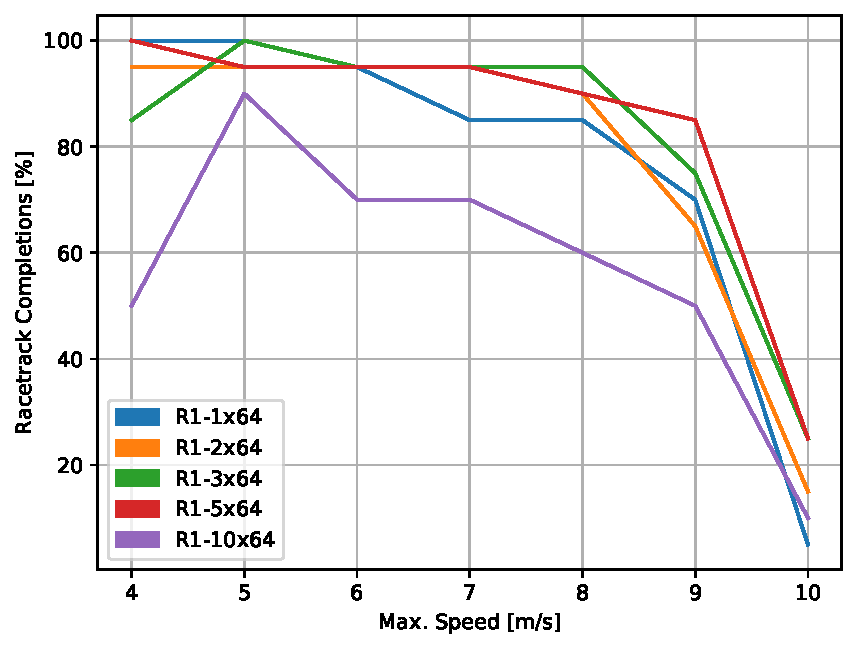
\includegraphics[width=\gfxwidth]{own/results_e2_racing.pdf}
    \caption[
        Racetrack completion shares of experiment 2
    ]{
        Racetrack completion shares of experiment 2
    \label{fig:e2_rcs}}
\end{figure}
R1-1x64, R1-2x64, R1-3x64 and R1-5x64
have roughly the same RCS,
which ranges from 85 to 100\%
for maximum speeds from 4 to 8 m/s,
from 65 to 85\% for 9 m/s and 
from 5 to 25\% for 10 m/s.
For maximum speeds from 9 to 10 m/s, however,
the RCS of R1-3x64 and R1-5x64 is approximately 10 percentage points higher than R1-1x64, R1-2x64.
Except for the maximum speed of 10 m/s,
R1-10x64 has the by far the lowest RCS,
which is about 20 percentage points lower over the tested maximum speeds.



%\paragraph*{Experiment 3}
Table \ref{tab:e3_data} shows
the data aggregation statistics of the imitation learning process for the variants of experiment 3.
\begin{table}[h]
    \caption[
        Data aggregation of experiment 3
    ]{
        Data aggregation of experiment 3
        \label{tab:e3_data}}        
    \centering
    \begin{tabular}{|c|r|r|} 
        %\hline
        \cline{2-3}
        \multicolumn{1}{c|}{}
        &E3F
        &E3R
        \\\hline
        %
        Learning completed
        &Yes
        &Yes
        \\\hline
        \# Rollouts
        &547
        &840
        \\\hline
        \# Training samples
        &25,470
        &40,216
        \\\hline
        \# Validation samples
        &None
        &None
        \\\hline
    \end{tabular}
\end{table}
Both variants, the feedforward and the recurrent variant, completed the imitation learning process.
Neither variant aggregated validation data 
because this feature had not yet been implemented when experiment 3 was conducted.
The feedforward variant (E3F) performed fewer rollouts with 547
and aggregated fewer data with 25,470 training samples
than the recurrent variant (E3R) which rolled out 840 times
and aggregated 40,216 training samples.

Figure \ref{fig:e3_learn} shows the 
training losses over the epochs of the imitation learning process for the variants of experiment 3.
\begin{figure}
    \centering
    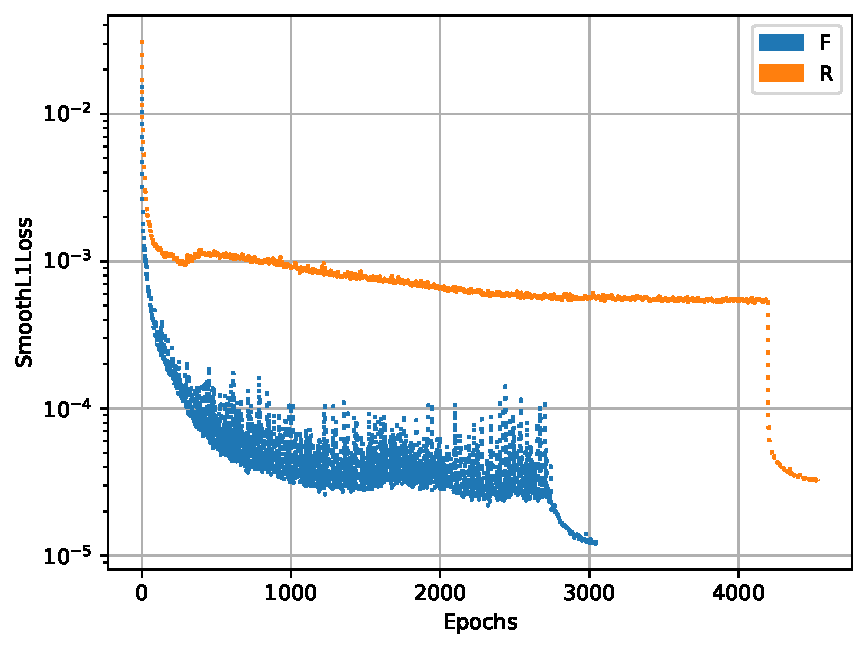
\includegraphics[width=\gfxwidth]{own/results_e3_learning.pdf}
    \caption[
        Training losses of experiment 3
    ]{
        Training losses of experiment 3
    \label{fig:e3_learn}}
\end{figure}
The training loss of a variant is calculated with the SmoothL1Loss function
on the training dataset aggregated by that variant.
E3F trained for fewer epochs with approximately 3000
and achieved a lower final training loss of $1.3\times 10^{-5}$
than E3R with approximately 4500 and $3.2\times 10^{-5}$.
In contrast to experiment 1 (see figure \ref{fig:e1_learn}),
the variants of experiment 3
continued to train
after the imitation learning process was completed 
until the training loss converged.
This can be recognized by the smoother curves at the end of the loss trends.
E3R makes a larger loss drop there
because the value of the dropout probability for a single application
had to be corrected to achieve a resultant dropout probability of 50\% for both variants.
The training loss trend of E3F fluctuates stronger than E3R
during the imitation learning process.


Figure \ref{fig:e3_racing} shows the 
RCS over the maximum drone speeds
of the race tests for the variants of experiment 3.
\begin{figure}
    \centering
    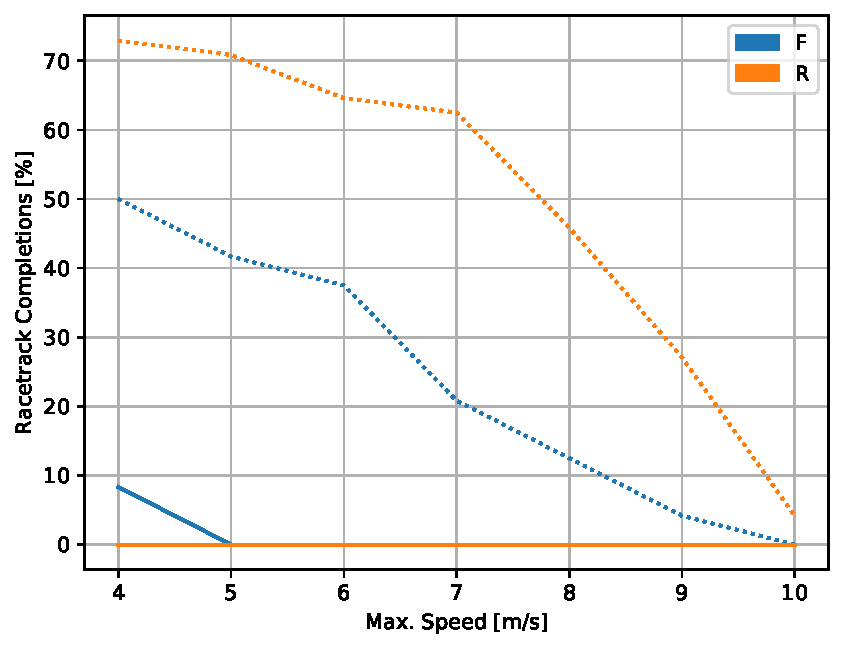
\includegraphics[width=\gfxwidth]{own/results_e3_racing.pdf}
    \caption[
        Racetrack completion shares of experiment 3
    ]{
        Racetrack completion shares
        for simulation environments
        seen (dotted) and unseen (solid) during learning
        of experiment 3
    \label{fig:e3_racing}}
\end{figure}
Thereby, the figure 
distinguishes between simulation environments seen and unseen in the imitation learning process.
In unseen environments, both variants have a RCS of about 0\% over all maximum speeds.
In seen environments,
E3R has a significantly higher RCS than E3F over the tested maximum speeds.
The RCS of E3F decrease almost linearly from 50\% for 4 m/s
to 0\% for 10 m/s.
The RCS of E3R ranges from 63 to 73\% for maximum speeds from 4 to 7 m/s
and, from there, decreases almost linearly to 5\% at 10 m/s.





%\paragraph*{Experiment 4}
Figure \ref{fig:e4_learn} shows the 
training losses over the epochs of the supervised learning process for the variants of experiment 4.
\begin{figure}
    \centering
    \subfloat[
        360x240 RGB images
    ]{
        \label{fig:e4_learn_feedforward_360x240}
        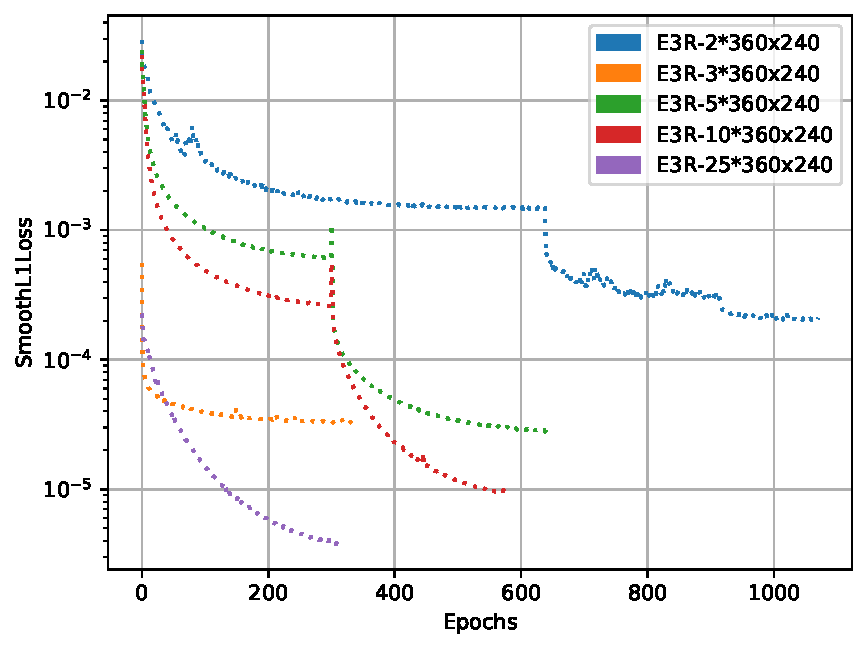
\includegraphics[width=\gfxwidth]{own/results_e4_learning_360x240.pdf}
    }
    \hspace*{0cm}
    \par
    \subfloat[
        240x160 RGB images
    ]{
        \label{fig:e4_learn_recurrent_240x160}
        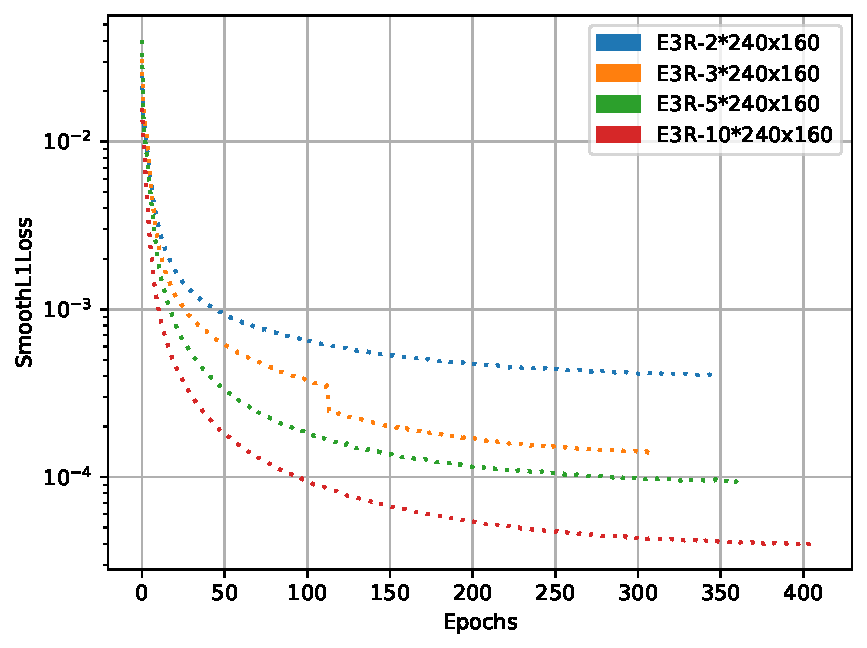
\includegraphics[width=\gfxwidth]{own/results_e4_learning_240x160.pdf}
    }
    \caption[
        Training losses of experiment 4
    ]{
        Training losses of experiment 4
        \label{fig:e4_learn}
    }
\end{figure}
%\begin{figure}
%    \centering
%    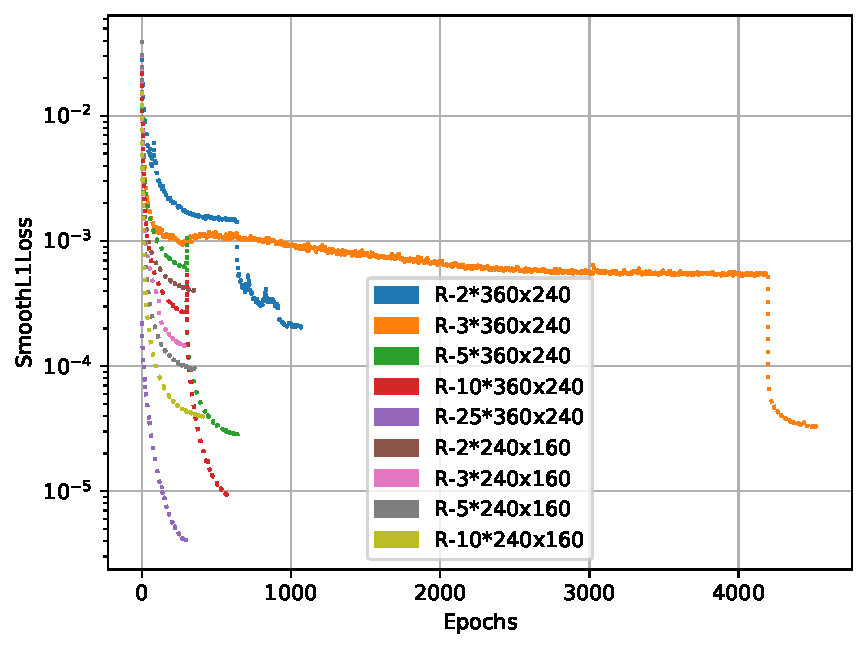
\includegraphics[width=\gfxwidth]{own/results_e4_learning.pdf}
%    \caption[
%        Training losses of experiment 4
%    ]{
%        Training losses of experiment 4
%    \label{fig:e4_learn}}
%\end{figure}
The training loss of a variant is calculated 
with the SmoothL1Loss function
on the final training dataset of E3R in experiment 3.
All variants trained close to convergence.
Drops in the loss trends trace back to corrections
of the dropout probability for a single application
to achieve a resultant dropout probability of 50\% for all variants.
The variants with the RGB image size of 360x240 
have lower training losses than their counterparts 
with the RGB image size of 240x160.
For both RGB image sizes, the longer the input sequence length 
of the training samples, the lower the training loss.
The loss trend of E3R-2*360x240 fluctuates stronger than for the other variants.




Figure \ref{fig:e4_racing} shows the
RCS over the maximum drone speeds
of the race tests of experiment 4.
\begin{figure}
    \centering
    \subfloat[
        RGB image size of 360x240
    ]{
        \label{fig:e4_racing_360x240}
        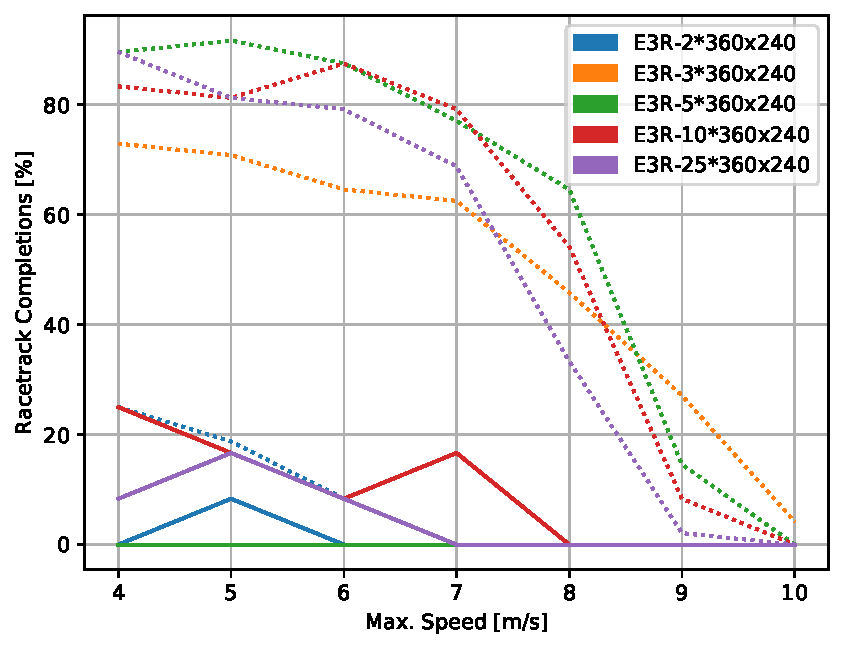
\includegraphics[width=\gfxwidth]{own/results_e4_racing_360x240.pdf}
    }
    \hspace*{0cm}
    \par
    \subfloat[
        RGB image size of 240x160
    ]{
        \label{fig:e4_racing_240x160}
        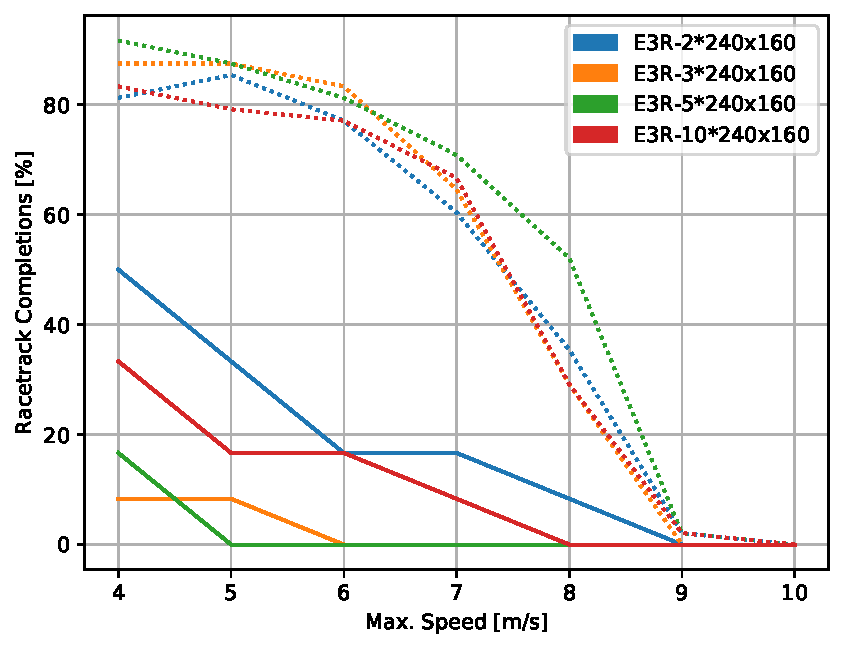
\includegraphics[width=\gfxwidth]{own/results_e4_racing_240x160.pdf}
    }
    \caption[
        Racetrack completion shares of experiment 4
    ]{
        Racetrack completion shares of experiment 4
        \label{fig:e4_racing}
    }
\end{figure}
%\begin{figure}
%    \centering
%    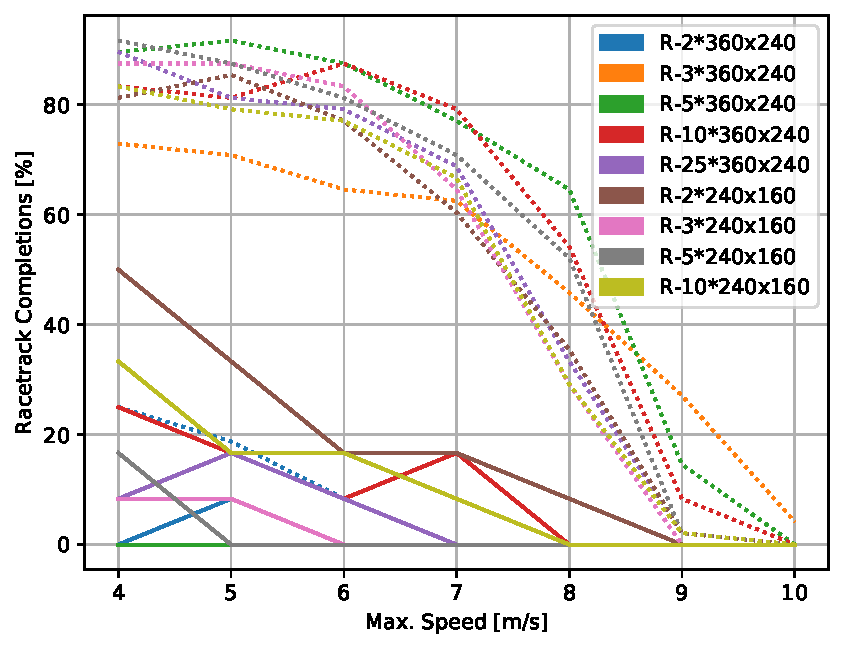
\includegraphics[width=\gfxwidth]{own/results_e4_racing.pdf}
%    \caption[
%        Racing test results of experiment 4
%    ]{
%        Share of completed racetracks dependent on the maximum drone speed 
%        during the racing tests of the ANN module variants of experiment 4.
%    \label{fig:e4_racing}}
%\end{figure}
The figure distinguishes between simulation environments seen and unseen in the imitation learning process.
In unseen environments,
all variants have an RCS close to 0\%,
except for E3R-10*360x240, E3R-25*360x240, E3R-2*240x160 and E3R-10*240x160,
whose RCS is up to 25, 20, 50, 35\% for maximum speeds up to 7, 6, 8, 7 m/s, respectively.
In seen environments,
all variants have roughly the same RCS over the tested maximum speeds,
which from about 80 to 90\% for 4 m/s decreases
almost parabolically to 0 to 15\% at 9 m/s.
Thereby, two variants stand out.
The RCS of the starting point variant (E3R-3*360x240) 
is slightly lower at lower maximum speeds from 4 to 7 m/s 
and a slightly higher at higher speeds from 9 to 10 m/s
and the RCS of E3R-2*360x240 is below 25\% for all tested maximum speeds.






%###################################################################################
%###################### Discussions         ########################################
%###################################################################################
\section{Discussions}
\label{discussions}
This section discusses and interprets the experimental results presented in the previous section. 
The performance of the ANN module variants is evaluated based on the data aggregation statistics 
and the loss trends from the learning process, as well as the racetrack completion shares (RCS) over maximum drone speeds 
from the race tests. The symbol $\sim$ denotes that a number is an approximate value.

Experiment 1 compares the variants by their learning ability for generalization to the randomized figure-8 racetrack 
in a fixed simulation environment. 
The layout of the figure-8 racetrack places three demands on navigation: 
the autonomous navigation method must be able to fly the drone through both, left and right, turns 
and across intersections. Intersections are especially difficult, 
because multiple gates appear in the drone's field of view, which can lead to ambiguities 
in the navigation decision-making.


The first feedforward variant of experiment 1 (F1), 
which resembles the ANN of the baseline work, 
could not learn these navigational qualities required by the figure-8 racetrack. 
As F1 stopped making progress, the imitation learning process of F1 was terminated. 
In the incomplete learning process, F1 still collected about three times more data than the other variants of experiment 1, 
with $\sim 76$k training samples. 
Nonetheless, F1 performed by far the worst in the race tests of experiment 1 
with a RCS of only $\sim 50\%$ for maximum speeds $\le 6$ m/s and $0\%$ for maximum speeds above. 
This poor performance of F1 contrasts with the results from the simulated experiments of the baseline work 
on a static racetrack and a dynamic racetrack with sinusoidally moving gates. 
On the static racetrack, the baseline method aggregated $\sim 74\%$ fewer training samples than F1 
but completed the racetrack at 100, $\sim 85$, $\sim 65$ and $\sim 30\%$ 
for maximum speeds $\le 9$ and of 10, 11 and 12 m/s, respectively. 
The by far worse race test performance of F1 could be attributed 
to the more difficult learning and testing conditions in experiment 1. 
While the baseline method rolls out on the same deterministic racetrack, 
F1 faces a slightly different randomized racetrack at each rollout in the imitation learning process and the race tests. 
However, considering the baseline results on the dynamic racetrack, 
this cannot be the only reason for the performance drop of F1. 
For learning to navigate through the dynamic racetrack, 
the baseline method rolled out on randomized racetracks like in experiment 1, 
whereby it collected $\sim 32\%$ more training samples than F1. 
At the race tests, the baseline method completed the dynamic racetrack with not too large gate movement amplitudes 
at $100\%$ for a maximum speed of 8 m/s. 
In contrast, F1 did not complete a single racetrack for maximum speeds $\le 7$ m/s, 
even though it performed the race tests on only static racetracks. 
The fact that F1 collected fewer data than the baseline method cannot explain the performance difference because first, 
F1 already stalled in the imitation learning process and second, 
the other variants of experiment 1 performed significantly better than F1 even though they collected by far fewer data. 
The main reason for the performance difference is likely the different layouts of the racetrack. 
The racetrack of the baseline work consists of 8 gates arranged in a circle, 
which requires the baseline method of only learning to fly the drone through either left or right turns. 
In contrast, F1 must deal with turns of both directions and intersections of the figure-8 racetrack. 
Another reason could be that the simulation of this thesis is more photo-realistic 
than the simulation in the baseline work. The low complexity of the Resnet8 integrated 
with the baseline ANN and F1 may only infer sufficiently from the less detailed, non-photorealistic 
images of the baseline simulation. 
This argument is supported by the fact that the other variants of experiment 1, 
which all integrate the more complex Resnet14, perform significantly better than F1. 
There is another distinguishing factor in experiment 1 from the baseline experiments: 
F1 inputs RGB images with the size of 240x160, whereas the baseline ANN of 300x200. 
However, the results of experiment 4, which examined variants of two image sizes, 
suggest that this slight difference in the image size has, if at all, only a marginal impact on the race test performance.



The second feedforward variant of experiment 1 (F2), 
which differs from F1 in integrating the more complex Resnet14 instead of the Resnet8, 
also stalled in the imitation learning process but performs significantly better than F1 in the race tests. 
F2 achieved an RCS from $\sim 60$ to $\sim 80\%$ for maximum speeds $\le 8$ m/s and $\sim 0\%$ for maximum speeds above. 
Considering that the final training and validation losses of F1 and F2 are almost equal, 
the question arises why F2 outperforms F1 in the race tests, 
especially since F2 aggregated $\sim 62\%$ fewer training samples than F1. 
The answer is that F1 stalled at about 2/3 of the rollout combinations of the imitation learning process, 
while F2 stalled only at the very last combination. 
Thus, the training and validation data aggregated by F2, 
although containing much fewer samples, represent the state distribution at the rollouts of the race tests more closely. 
The early stages of the learning process, where the data quantity and quality are more comparable, 
show that F2 can reduce the training and the validation loss more and faster than F1. 
Overall, the comparison of F1 and F2 finds that a more complex CNN architecture 
can learn more accurately (lower losses on comparable data, same losses on more comprehensive data) 
and effectively (fewer rollouts/epochs and data) 
in the imitation learning process, 
which results in significantly better performance in the race tests. 
This comparison does not consider whether a drone with limited computational power 
could run the more complex network at the required frequency.



The first recurrent variant of experiment 1 (R1) differs 
from F2 in integrating three GRU instead of three fully-connected layers. 
R1 completed the imitation learning process in contrast to F2, 
whereby R1 aggregated $\sim 38\%$ fewer training samples and $\sim 45\%$ fewer rollouts. 
This shows that R1 needs substantially fewer data to learn a more accurate 
navigation decision-making than F2. Because rollouts are costly and dangerous in the 
real-world, R1 is more workable in real-world imitation learning than F2. Considering 
that the recurrent variants trained for only three while the feedforward variant trained 
for ten epochs per rollout, R1 could further reduce the data and number of rollouts in 
the comparison with F2. However, this would make the learning process of R1 much more 
time-consuming compared to F2, since the samples of R1 have an input sequence of 25 RGB 
images, while the samples of F2 have only a single RGB image input. 
In $\sim 83\%$ fewer epochs, R1 achieved a $\sim 91\%$ lower final training loss 
and a $\sim 95\%$ lower 
final validation loss than F2. This results in a $\sim 42\%$ lower validation-training loss 
ratio of R1, while both variants have a resultant dropout probability of 
$50\%$ during training. 
The much lower losses of R1 suggest that a navigation decision is indeed temporally 
related to past visual observations from the drone's onboard camera and that R1, 
as it is recurrent, learns to leverage these underlying temporal connections for a more 
accurate navigation decision-making. The lower validation-training loss ratio of R1 suggests 
further that incorporating these temporal connections abstracts the navigation 
decision-making more and thus enhances the generalization ability of R1. R1 could 
transfer its better learning performance to a better race test performance. The RCS of 
R1 is $\sim 20$ percentage points higher than F2 for maximum speeds from 5 to 8 m/s and $\sim 55$ 
percentage points for a maximum speed of 9 m/s. Overall, the comparison of F2 and R1 
indicates that the combined spatial and temporal (instead of a mere spatial) comprehension 
of the visual perception increases the performance of the autonomous navigation method for 
learning and testing on the randomized figure-8 racetrack. Considering that the variants of 
experiment 1 make navigation decisions at 50 Hz, R1 learns to memorize what it has seen for 
a time span of 0.5 s from the training on input sequences with a length of 25. In other words, 
R1 bases its navigation decision-making on 0.5 s videos, while F2 bases it on single images. 
Unlike a single frame, a video encodes the drone's latest motion sequence relative to the 
racetrack and the environment. This information could, for example, resolve the ambiguities 
stemming from the intersections of the figure-8 racetrack or render the decision-making more 
robust against single outlier frames that differ significantly from the aggregated training data.



%In order to be able to make conclusive statements about the use of the optional inputs, more experiments must be conducted. The margin-threshold pairs of the learning configuration could be configured more stringent, whereby a variant would be forced to collect more data to complete the learning process. As a result, the validation-training loss ratio of R2 could become closer to R1 and R2 could outperformR1 in the race tests.
%Further experiments could be conducted to investigate whether variants with a trainable CNN submodule could reduce overfitting with stronger regularization of the CNN submodule and whether a thereby reduced overfitting would reflect in the race test performance.
%Further experiments could investigate whether R1-10x64 in the imitation learning process could leverage its greater depth on its self-aggregated data to outperform the other variants.

The second recurrent variant of experiment 1 (R2) differs from R1 in the additional 
use of the optional inputs (i.e., time increment of RGB images, IMU data with time increment). 
R2 completed the imitation learning process with $\sim 19\%$ more rollouts and $\sim 15\%$ 
more training 
samples than R1. In $\sim 15\%$ more epochs, R2 achieved a $\sim 33\%$ 
lower final training loss but
a $\sim 679\%$ higher final validation loss than R1. This results in a $\sim 1063\%$ higher, 
validation-training loss ratio than R1, while both variants have a resultant dropout probability 
of $50\%$ during training. The lower training loss of R2 suggests that the optional inputs are 
related to the navigation decisions and R2 learns to use these relations. For example, R2 could 
have learned to weigh the incoming images with their time increment information or to refine 
the drone's motion history with the incoming IMU data. However, the by far larger 
validation-training loss ratio shows that R2 heavily overfits its aggregated training data, 
which reflects in the race test performance. The RCS of R2 is $\sim 20$ percentage points lower 
than R1 for maximum speeds from 5 to 9 m/s. The reason for the overfitting could be that 
combining both the visual and physical features in the data from the drone's onboard camera 
and IMU, respectively, increases the variance of the decision-making basis enormously. 
As a result, R2 would 
require much more training data than R1 for generalization. R2 could overcome its overfitting 
on more training data, whereby it possibly could outperform R1 in the race tests.



The third recurrent variant of experiment 1 (R3)
differs from R1 in the fact that 
the Resnet14 was pretrained 
and only partly trainable in the learning process.
This was a successful attempt to speed up the time of a training epoch.
However, it made the training less effective,
whereby the imitation learning process took more rollouts and epochs,
which canceled the time advantage.
R3 completed the imitation learning process with $\sim 56\%$ more rollouts
and $\sim 55\%$ more training samples than R1.
In $\sim 57\%$ more epochs,
R3 achieved a $\sim 641\%$ higher final training loss
and a $\sim 144\%$ higher final validation loss than R1.
This results in a $\sim 66\%$ lower validation-training loss ratio 
than R1, 
while both variants have a resultant dropout probability of $50\%$ during training.
R3 cannot benefit from the low ratio and transfers the significantly higher losses to the race tests,
where it performs $\sim 30$ percentage points worse than R1 at the maximum speeds from 5 to 9 m/s.
The very little validation-training loss ratio of R3 
indicates that R3 does basically not overfit.
Looking at the loss trends of R3,
one can see that the trainings with the CNN submodule trainable
drastically reduce the losses but also increase the validation-training loss ratio,
while the trainings with the CNN module not trainable
slightly reduce the losses and also the validation-training loss ratio.
This could mean that the overfitting of the other variants of experiment 1
mainly stem from the CNN submodule.


At a maximum speed of 9 m/s, all three recurrent variants perform better than the feedforward variants.
It is therefore likely that the higher the speed, the more beneficial the memory capabilities become for
the navigation decision-making.
One explanation could be that higher speeds require higher accelerations,
which in turn require the drone to lean more into turns.
Therewith, the drone's onboard camera could produce more outlier images
and the above mentioned ability to recall past images 
to compensate for outlier images would thus be even more valuable.
Another explanation could be that the memory time span is fixed at 0.5 s for the recurrent variants.
The higher the speed, the further the memory expands spatially.
This could make the memory more meaningful in terms of the drone's motion sequence in the racetrack.



Experiment 2 varies R1 from experiment 1 
with respect to the number of GRU layers in order to investigate the impact of the 
GRU submodule's depth on the performance of a variant. 
Because of the high time expenditure of the imitation learning process, 
the variants of experiment 2 only train and validate with supervised learning on the 
final dataset aggregated by R1 in experiment 1. 
All variants trained for 200 epochs, whereby the training losses did not fully converge 
while the validation losses almost converged. The number of GRU layers had only 
a negligible influence on the epoch time, which is likely dominated by the loading 
of the sequential training data from disk.
The fact that the ten-layer GRU variant (R1-10x64)
has a $\sim 77\%$ higher training
but a $\sim 35\%$ lower validation loss 
than the other multi-layer GRU variants (R1-2x64, R1-3x64 and R1-5x64)
shows that the formula used to calculate the single application dropout probability
for a resultant dropout probability of $50\%$ is only an approximation.
The single-layer GRU variant (R1-1x64) falls out of this comparison as it has no dropout.
At the race tests, R1-1x64, R1-2x64, R1-3x64 and R1-5x64 performed equally well.
They completed the racetrack at $\sim 85 - 100\%$ for maximum speeds of 4 to 8 m/s,
at $\sim 65 - 85\%$ for 9 m/s 
and at $\sim 5 - 25\%$ for 10 m/s.
R1-3x64 and R1-5x64 exhibit a slightly better performance at higher maximum speeds of 9 and 10 m/s.
R1-10x64 performed significantly worse, 
with $\sim 20$ percentage points fewer over the tested maximum speeds.
Compared to the equally configured but less trained out R1 in experiment 1,
R1-3x64 achieved a $\sim 41\%$ lower final training
and a $\sim 16\%$ higher final validation loss
and performed slightly better over all tested maximum speeds.
For the comparisons of R1-10x64 vs. R1-1x64, R1-2x64, R1-3x64 and R1-5x64
as well as R1 vs. R1-3x64,
the worse performing variant has a higher final training loss and a lower final validation loss.
The training loss, thus, seems to be more important for the race test performance than the validation loss.
One reason for this could be the way data is aggregated in the imitation learning process.
The training and the validation dataset are basically a collection of mistakes made in the learning rollouts.
The fully trained variant likely avoids a lot of drone states, 
for which the validation dataset provides a correct navigation decision,
in the first place.
An important insight from experiment 2 is that 
the further training of a variant, after it completed the imitation learning process,
likely enhances the race test performance.
While experiment 2 cannot make clear statements,
whether more GRU layers are generally more capable in the autonomous navigation method,
it suggests the use of R1-3x64 and R1-5x64 over R1-1x64 and R1-2x64.
However, the worst performing R1-10x64
could leverage its greater depth 
in the imitation learning process
to outperform the other variants.



Experiment 3 focuses on the learning ability of a variant for generalization 
to the randomized gap racetrack in simulation environments seen an unseen in the 
imitation learning process. The layout of the gap racetrack places two demands on 
the autonomous navigation method, i.e., to fly through left or right turns and through 
the gap. The gap is extremely challenging because when flying through it, there is 
intermediately no gate in the drone's field of view (FOV). A feedforward ANN module could 
only learn to pass the gap by using visual information in seen environments. A recurrent 
ANN module could also learn to pass the gap in unseen environments by recalling 
past visual information from its memory. Before the drone enters the gap, both gates 
surrounding the gap appear in the drone's FOV. As soon as the drone enters the gap and the 
FOV becomes gate-free, the ANN module could implicitly localize the next gate relative to the 
drone from its memory in order to make meaningful navigation decisions towards that gate. 
Even if the memory time span is too short to cover the entire time span in which the FOV is 
gate-free, after initializing the left or right turn in the covered time span, the drone could 
have the memory-based awareness that it is flying a left or right turn and 
could maintain the turn for the uncovered time span until the next gate reappears in the FOV. 

Experiment 3 studies a feedforward variant (E3F) and a recurrent variant (E3R).
E3F completed the imitation learning process
with $\sim 35\%$ fewer rollouts and $\sim 37\%$ fewer training samples than E3R.
Moreover, E3F
trained for $\sim 33\%$ fewer epochs and  
achieved a $\sim 59\%$ lower final training loss than E3R.
The better learning performance of E3F compared to E3R
is in contradiction with the results of experiment 1,
which could be explained by the fact
that the FC submodule of E3F has 
$\sim 818\%$ more trainable parameters than the GRU submodule E3R.
In experiment 3, unlike experiment 1 conducted later,
no attention was paid to ensure
that the FC and GRU submodules of the variants
were approximately equal in the number of trainable parameters.
Despite its worse learning performance,
E3R outperforms E3F in the race tests in seen environments
by $\sim 5 - 40\%$ percentage points over the tested maximum speeds.
In unseen environments,
both variants failed the race tests.
The performance difference in seen and unseen environments
suggests that both variants learned to use visual information in the environment to pass the gap.
The yet better race test performance in the seen environments of E3R compared to E3F
is consistent with the results and their interpretations of experiment 1.
Overall, experiment 3 failed to create the test conditions that would force the 
use of memory to navigate through the intermediate target loss of the gap.



Experiment 4 varies E3R from experiment 3 with respect to the input sequence length 
of the training samples and the size of the RGB images of the training samples and 
incoming at rollout in order to investigate their effects on performance. 
The variants of experiment 4 share the same learning capabilities, because their ANN 
modules are configured the same. However, the variants are provided with different 
resources to learn from. Like experiment 2, the variants of experiment 4 trained with 
supervised learning to save time. Each variant trained on its own training dataset, 
that had been rebuilt from the raw records of E3R with the corresponding sequence length 
and image size of that variant. All variants trained until near convergence. For variants 
of the same image size, the longer the sequence length, the lower the training loss of the 
variant. This substantiates the interpretation from experiment 1 that navigation decisions 
are temporally connected to past sensor data and that these connections are learnable by 
recurrent variants. For the range of investigated sequence lengths, the longer the memory 
time span, the more the variant can learn. For variants of the same sequence length, the 
larger the image size, the lower the training loss. This shows that a more detailed, visual 
observation is a stronger resource to learn the navigation decision-making. The race test 
performances of the variants are roughly the same, whereby lower training losses do not 
reflect in higher performances. The variants with the smaller image size perform slightly 
better in unseen environments than the variants with the bigger image size. A reason for 
this could be that, the ratio of spatial to temporal information in the training samples 
decreases with the image size, which favors the learning of temporal before spatial features, 
which are necessary to pass the gap in unseen environments as mentioned above.

%Experiment 4 varies E3R (from experiment 3)
%with respect to the input sequence length of the training samples
%and the input RGB image size at training and rollout
%in order to investigate their effects on performance.
%The variants of experiment 4 
%share the same learning capabilities, because their ANN modules are configured the same,
%but are provided with different resources to learn from.
%Due to the high time expenditure of the imitation learning process, 
%the variants of experiment 4 trained with supervised learning.
%Each variant trained on its own training dataset,
%that had been rebuilt from the raw records of E3R 
%with the corresponding sequence length and image size of that variant.
%All variants trained until near convergence.
%For variants of the same image size,
%the longer the sequence length,
%the lower the training loss of the variant.
%This substantiates the interpretation from experiment 1
%that navigation decisions are temporally connected to past sensor data
%and that these connections are learnable by recurrent variants.
%For the range of investigated sequence lengths,
%the longer the memory time span,
%the more the variant can learn.
%For variants of the same sequence length,
%the larger the image size, the lower the training loss.
%This shows that a more detailed, visual observation 
%is a stronger resource to learn the navigation decision-making.
%The race test performances of the variants are roughly the same,
%whereby lower training losses do not reflect in higher performances.
%The variants with the smaller image size perform 
%slightly better in unseen environments than the 
%variants with the bigger image size.
%A reason for this could be that, the ratio
%of spatial to temporal information in the training samples
%decreases with the image size,
%which favors the learning of temporal before spatial features,
%which are necessary to pass the gap in unseen environments as mentioned above.
%Further experiments
%could find whether a variant
%trained with imitation learning
%can leverage its lower training loss
%to achieve a better race performance.


































